\documentclass[10pt,a4paper,table]{article}
	
	\usepackage{amsmath,amssymb,amsthm,mathtools,amsfonts}
	\usepackage{breqn}
	\usepackage[utf8]{inputenc}
	\usepackage[danish]{babel}
	\usepackage[T1]{fontenc}
	
	%%%%%%%%%%%%%%%%%%%%%%%%%%%%%%%%%%%%%%%%%%%%%%%%%%%%%%%%%%%%%%%%%%%%%%%%%%%%%% Fonts
	
	\usepackage{fontspec}
	\setmainfont{Times New Roman}
	\newfontfamily\garamond[Numbers=OldStyle]{EB Garamond}
	\newfontfamily\plantin[Numbers=OldStyle]{Plantin MT Pro}
	\newfontfamily\wal{Walbaum Com}
	\newfontfamily\klav{Klavika}
	\newfontfamily\klavl{Klavika light}
	\newfontfamily\quotefont[Ligatures=TeX]{Linux Libertine O}
	\newfontfamily\vest{TRY Vesterbro Regular}
	\newfontfamily\vestb{TRY Vesterbro Poster}
	\newfontfamily\overp{Overpass}
	
	%%%%%%%%%%%%%%%%%%%%%%%%%%%%%%%%%%%%%%%%%%%%%%%%%%%%%%%%%%%%%%%%%%%%%%%%%%%%%% Colors
	
	\usepackage{xcolor}
	
	\definecolor{frbblue}{RGB}{47, 88, 109}
	\definecolor{hgred}{RGB}{140, 10, 10}
	\definecolor{frbgreenl}{RGB}{162, 202, 137}
	\definecolor{frbgreen}{RGB}{28, 85, 66}
	\definecolor{frbgrey}{RGB}{243, 245, 242}
	
	%%%%%%%%%%%%%%%%%%%%%%%%%%%%%%%%%%%%%%%%%%%%%%%%%%%%%%%%%%%%%%%%%%%%%%%%%%%%%% Other Graphics
	
	\usepackage{graphicx}
	\graphicspath{{../img/}}
	\usepackage{tikz}
	\usepackage{placeins}
	\usepackage{subcaption}
  \usepackage{float}
	
	\usepackage[pdfborder={0 0 0}]{hyperref} %% Ingen firkant rundt om referencer

	\usepackage{multicol}
	\usepackage{cellspace}
		\setlength\cellspacetoplimit{100pt}
		\setlength\cellspacebottomlimit{100pt}
	\usepackage{tabularx}
		\newcolumntype{b}{>{\hsize=\hsize}>{\centering\arraybackslash}X}
	\usepackage{siunitx}
	\usepackage{cellspace}
		\setlength\cellspacetoplimit{4pt}
		\setlength\cellspacebottomlimit{4pt}
	
	\usepackage{enumitem}% better controls with enumerating
	\usepackage{wrapfig}
	\usepackage{caption}
	%\usepackage{dirtytalk}
	%\usepackage{tasks}
	\usepackage{titlesec}

	\setlength{\parskip}{0.5\baselineskip}
	\setlength{\parindent}{0cm}
	\setlist[enumerate]{label=\alph*),left=20pt}
	%\setlist[enumerate]{leftmargin=\parindent}
	%\setlist[enumerate]{nosep}
	
	
	%%%%%%%%%%%%%%%%%%%%%%%%%%%%%%%%%%%%%%%%%%%%%%%%%%%%%%%%%%%%%%%%%%%%%%%%%%%%%% New commands
	
	\newcommand\svar[1]{\color{red}{#1}\color{black}}
	
	\usepackage[h]{esvect}
	\newcommand{\twvect}[2]{\ensuremath{\begin{pmatrix}#1\\#2\end{pmatrix}}}
	
	\newcommand*\quotesize{20}
	\newcommand*{\openquote}
		{\tikz[remember picture,overlay,xshift=-3ex,yshift=-0ex]
			\node (OQ) {\quotefont\fontsize{\quotesize}{\quotesize}\selectfont``};\kern0pt}

	\newcommand*{\closequote}[1]
		{\tikz[remember picture,overlay,xshift=2ex,yshift={#1}]
			\node (CQ) {\quotefont\fontsize{\quotesize}{\quotesize}\selectfont''};}
			
	\newcommand{\qm}[1]{``#1''}
	\newcommand{\iquote}[1]{\begin{quote}\itshape \openquote#1\hfill\closequote{0ex} \end{quote}}
	
	%%%%%%%%%%%%%%%%%%%%%%%%%%%%%%%%%%%%%%%%%%%%%%%%%%%%%%%%%%%%%%%%%%%%%%%%%%%%%% Sections
	\usepackage{chngcntr}
	
	\renewcommand\thesection{\arabic{section}}

	\titleformat{\section}[block] 
  		{\flushright\overp\Large\color{frbgreen}}    % format for whole title
  		{}                           % no separate label (empty)
  		{0pt}                        % spacing between label and title
		{DELPRØVE \thesection}       % prepend "Delprøve <number>"
		[{\color{frbgreenl}\vspace{-1em}\hspace*{-0.165\linewidth}\rule{\dimexpr1.165\linewidth\relax}{0.4pt}\kern1mm}]
	
	\counterwithout{subsection}{section}
	\renewcommand\thesubsection{Opgave \arabic{subsection}}
	\titleformat{\subsection}[leftmargin]{\bfseries}{}{0pt}{\hspace{-5em}\thesubsection}
	
	%%%%%%%%%%%%%%%%%%%%%%%%%%%%%%%%%%%%%%%%%%%%%%%%%%%%%%%%%%%%%%%%%%%%%%%%%%%%%% Header & Footer
	
	\usepackage{bigfoot}
	\DeclareNewFootnote{a}
		\renewcommand{\thefootnotea}{\fnsymbol{footnotea}}
			\newcommand{\footnotes}[1]{\footnotea[2]{#1}} % here you can specify what symbol you want in footnotes
			\MakePerPage{footnotes}
	
		\usepackage{fancyhdr}
	\fancypagestyle{plain}{%
		\setlength{\headheight}{60pt}%
		\setlength{\headsep}{0pt}
		\fancyhf{}% No header/footer
		\renewcommand{\footrulewidth}{0pt}% No footer rule
		\renewcommand\headrule{
			\centerline{\begin{minipage}{1\textwidth}
				\color{frbblue}\hrule width \hsize \kern 1mm \hrule width \hsize height 2pt \vspace{4em}
			\end{minipage}}
		}
		\fancyhead[L]{\hspace{0em}
\includegraphics[height=2.5em]{frbvuc_logo.png}}
		\fancyhead[R]{\overp\color{frbgreen}\footnotesize Forår 2026}
		\fancyhead[C]{\overp\color{frbgreenl}\normalsize \overp Mat C-B\\\Large\color{frbgreen}\vestb Vejledende opgavesæt: besvarelse}
		\cfoot{\thepage}
	}
	\pagestyle{fancy}
	\fancyhf{}
	\renewcommand\headrule{
			\centerline{\begin{minipage}{\textwidth}
				\color{frbgreen}\hrule width \hsize \kern 1mm
			\end{minipage}}}
	\lhead{\overp\color{frbgreen}\footnotesize Mat C-B}
	\rhead{\overp\color{frbgreen}\footnotesize Forår 2026}
	\cfoot{\thepage}
	
	%%%%%%%%%%%%%%%%%%%%%%%%%%%%%%%%%%%%%%%%%%%%%%%%%%%%%%%%%%%%%%%%%%%%%%%%%%%%%% Document

\begin{document}
\thispagestyle{plain}

\section{}
\subsection{}
\begin{enumerate}
  \item Vi løser ligningen ved at at
    \begin{enumerate}[label=\arabic*.]
      \item Gange 3 ind i parentesen
      \item Addere med to på begge sider af lighedstegnet
      \item Og til sidst dividere med 3 på begge sider af lighedstegent.
    \end{enumerate}
  \end{enumerate}

\begin{align*}
  3(x-2)&=15\\
  3x-6&=15\\
  3x&=21\\
  x&=7
\end{align*}

\begin{enumerate}[resume]
  \item Tallet 27 fortæller at medlemstallet i håndboldklubben stiger med 27 om året efter år 2020.
  \item De to linjer er ikke ortogonale da $-0,5\cdot 4\neq-1$.
  \item På grafen kan det ses at funktionen er faldende mellem $x$-værdierne 2 og 4. Intervallet hvor funktionen er faldende er derfor $[2;4]$.
  \end{enumerate}

\subsection{}
\begin{enumerate}
  \item Vi reducerer ved at bruge kvadratsætningen på parentesen og samle $a$'er og tal: $$a^2 + 3^2 + 2\cdot a \cdot 3 - 6a + 1 = a^2 + 10 $$
\end{enumerate}

\subsection{}
\begin{enumerate}
  \item Tallet $p$ kan bestemmes ved at trække alle talle fra 1:
    $$p=1-0,6-0,2-0,1=0.1$$
  \item Vi bruger formlen fra formelsamlingen: $$E(X)=0,6\cdot 10 + 0 0,2\cdot20 + 0,1\cdot 30 + 0,1 \cdot 40 = 17$$
\end{enumerate}

\subsection{}
\begin{enumerate}
  \item $f'(x)=4x^3-2x$
  \item \begin{align*}
      f(1)&=1^4-1^2+3=3\\
      f'(1)&=4\cdot1^3 - 2\cdot 1=2
    \end{align*}
  \item $f(1)$ er $y$-værdien når $x=1$ og $f'(1)$ er hældningen af tangenten når $x=1$:

\FloatBarrier
    \begin{figure}[H]
\centering
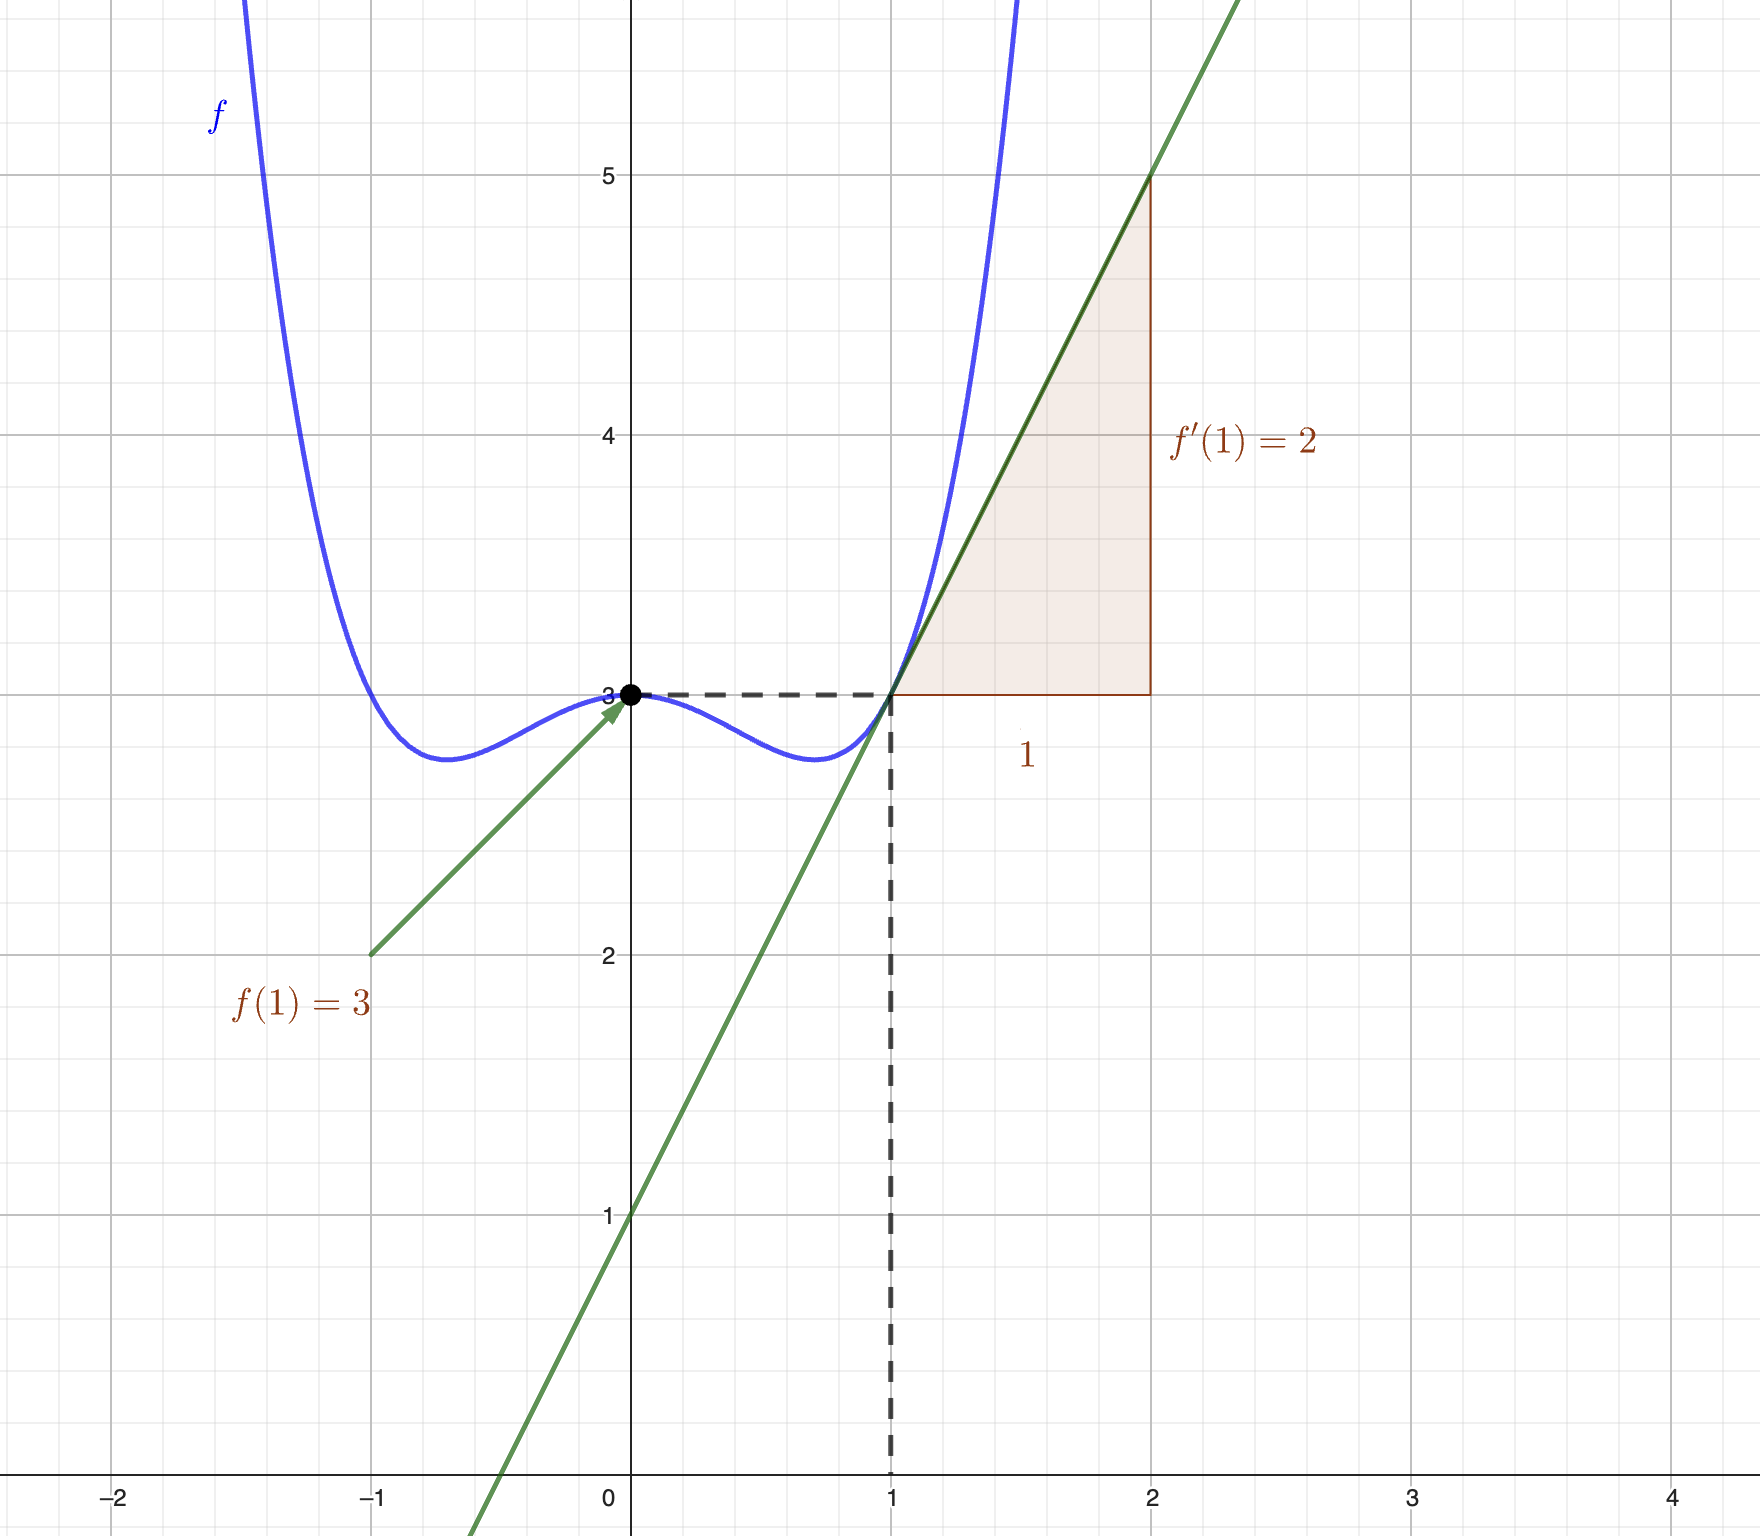
\includegraphics[width=0.6\textwidth]{værdier.png}
\end{figure}

\end{enumerate}

\subsection{}
\begin{enumerate}
  \item Da punktet ligger på grafen må $f(x)$ i forskriften være $$f(x)=5$$ og $x$ i forskriften $$x=2$$ indsætter vi disse værdier får vi en ligning som vi kan løse for at bestemme $c$:

    \begin{align*}
      f(x)&=x^2-3x+c\\
      5&=2^2-3\cdot 2+c\\
      5&=4-6+c\\
      5&=-2+c\\
      7&=c
    \end{align*}

    Altså må $c=7$.

  \end{enumerate}

  \subsection{}
  \begin{enumerate}
  \item At $a=0,5$ betyder at grenene for parablen vender opad, og at $d<0$ betyder at parablen ikke skærer $x$-aksen nogen steder. Det kan godt være figur 1, da denne parabel opfylder begge disse ting; det kan ikke være figur 2, da denne parabels grene vender nedad; det kan heller ikke være figur 3, da denne parabel skærer $x$-aksen to steder.
  \end{enumerate}

  \subsection{}
  \begin{enumerate}
    \item I skæringspunktet med $x$-aksen er $y$-værdien $y=0$. Indsætter vi denne værdi i cirklens ligning får vi en ligning som vi kan løse for at bestemme fsrstekoordinaten, eller $x$-værdien:

      \begin{align*}
        x^2+(y+2)^2&=13\\
        x^2+(0+2)^2&=13\\
        x^2+2^2&=13\\
        x^2+4&=13\\
        x^2&=13-4\\
        x^2&=9\\
        x&=\sqrt{9}\\
        x&=\pm3
      \end{align*}

Førstekoordinaten til cirklens skæringspunkter med $x$-aksen er derfor $x=3$ og $x=-3$.

    \end{enumerate}

    \section{}
    \subsection{}
    \begin{enumerate}
      \item Tallene kan bestemmes ved at indsætte tallene fra tabellen i geogebra's regneark og vælge funktionen "to-variabel analyse" og den polynomielle model. Her får man forskriften: $$f(x)=-5.1276x^2+186.8938x+8466.7891$$. Her kan vi aflæse $a$-, $b$-, og $c$-værdierne til  
        \begin{align*}
          a&=-5.1276\\
          b&=186.8938\\
          c&=8466.7891
        \end{align*}

      \item I modellen er højden bestemt ved $f(x)$. Det er altså grafen for denne funktions maximum vi skal finde. I geogebra kan man kopiere funktionen fra regressionsanalysen ind i grafvinduet. Herefter kan finde parablens toppunkt ved at bruge menuen i toppen:


\begin{figure}[H]
\centering
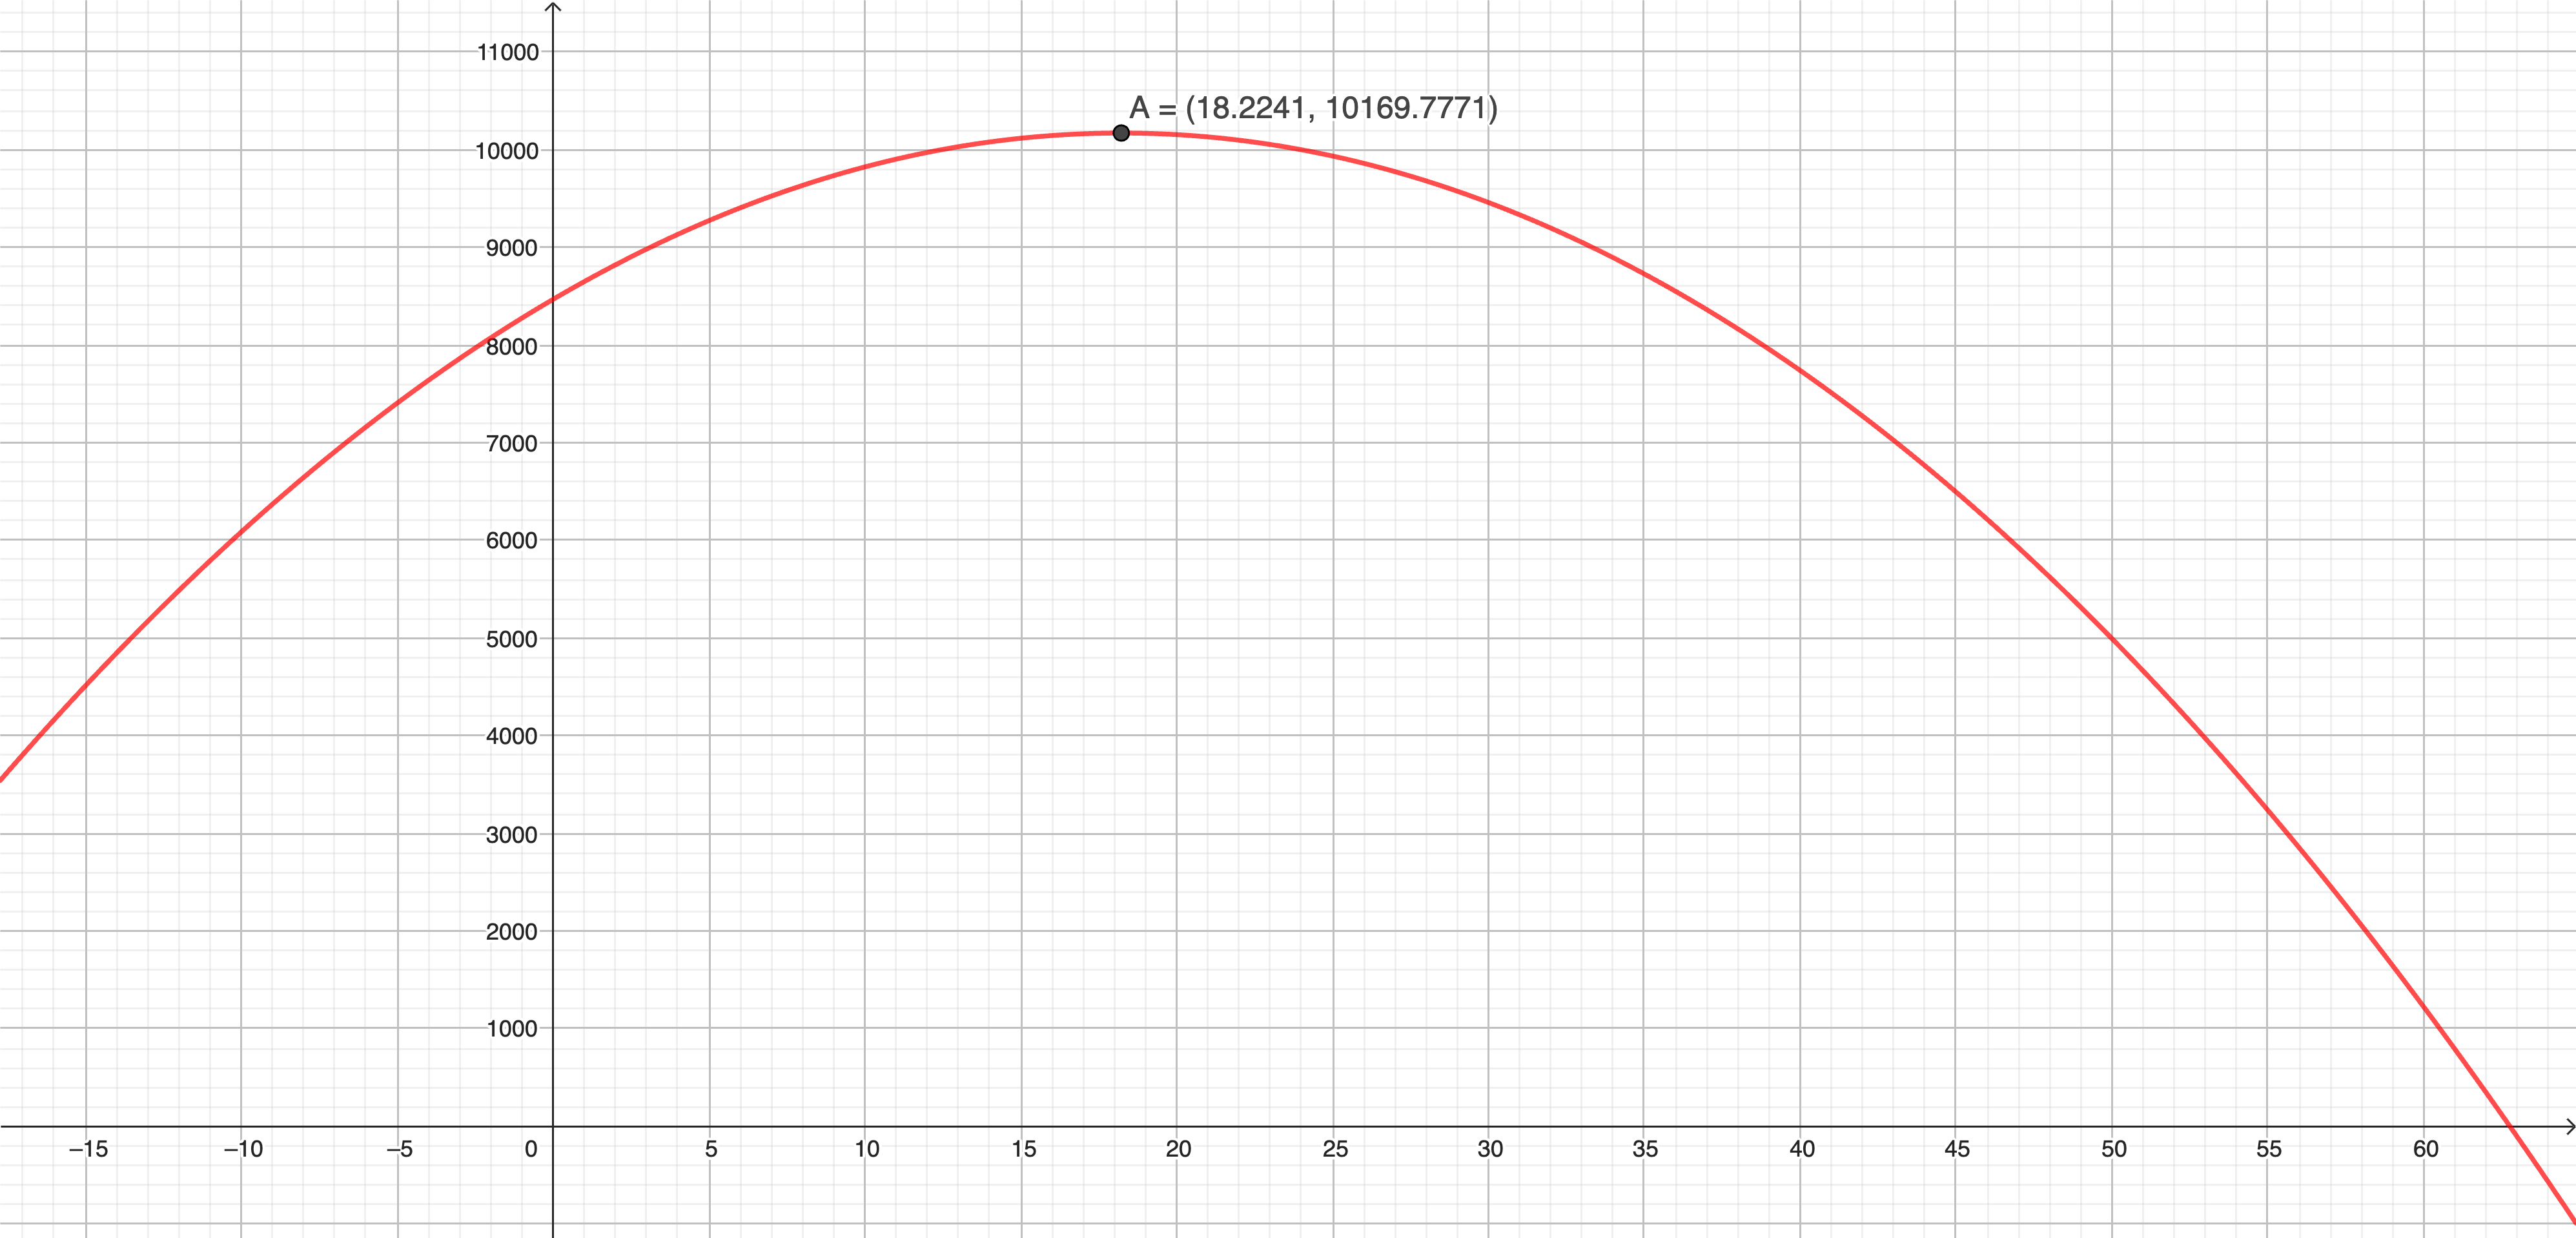
\includegraphics[width=0.6\textwidth]{toppunkt.png}
\end{figure}

Den maksimale højde er altså $10169,7771$.

      \end{enumerate}

      \subsection{}
      \begin{enumerate}
        \item I formelsamling er formel nummer (49) en formel for halveringstiden i denne type funktion:
      $$T_{\tfrac12}=\frac{\ln\left(\tfrac12\right)}{k}$$
      I funktionen $f(x)=200\cdot \text{e}^{-0,0103x}$ er $k=-0,0103$. Halveringstiden bliver derfor:
      $$T_{\tfrac12}=\frac{\ln\left(\tfrac12\right)}{-0,0103}\approx 67,3$$

    \item I geogebras CAS vindue kan man udregne værdien:

\begin{figure}[H]
\centering
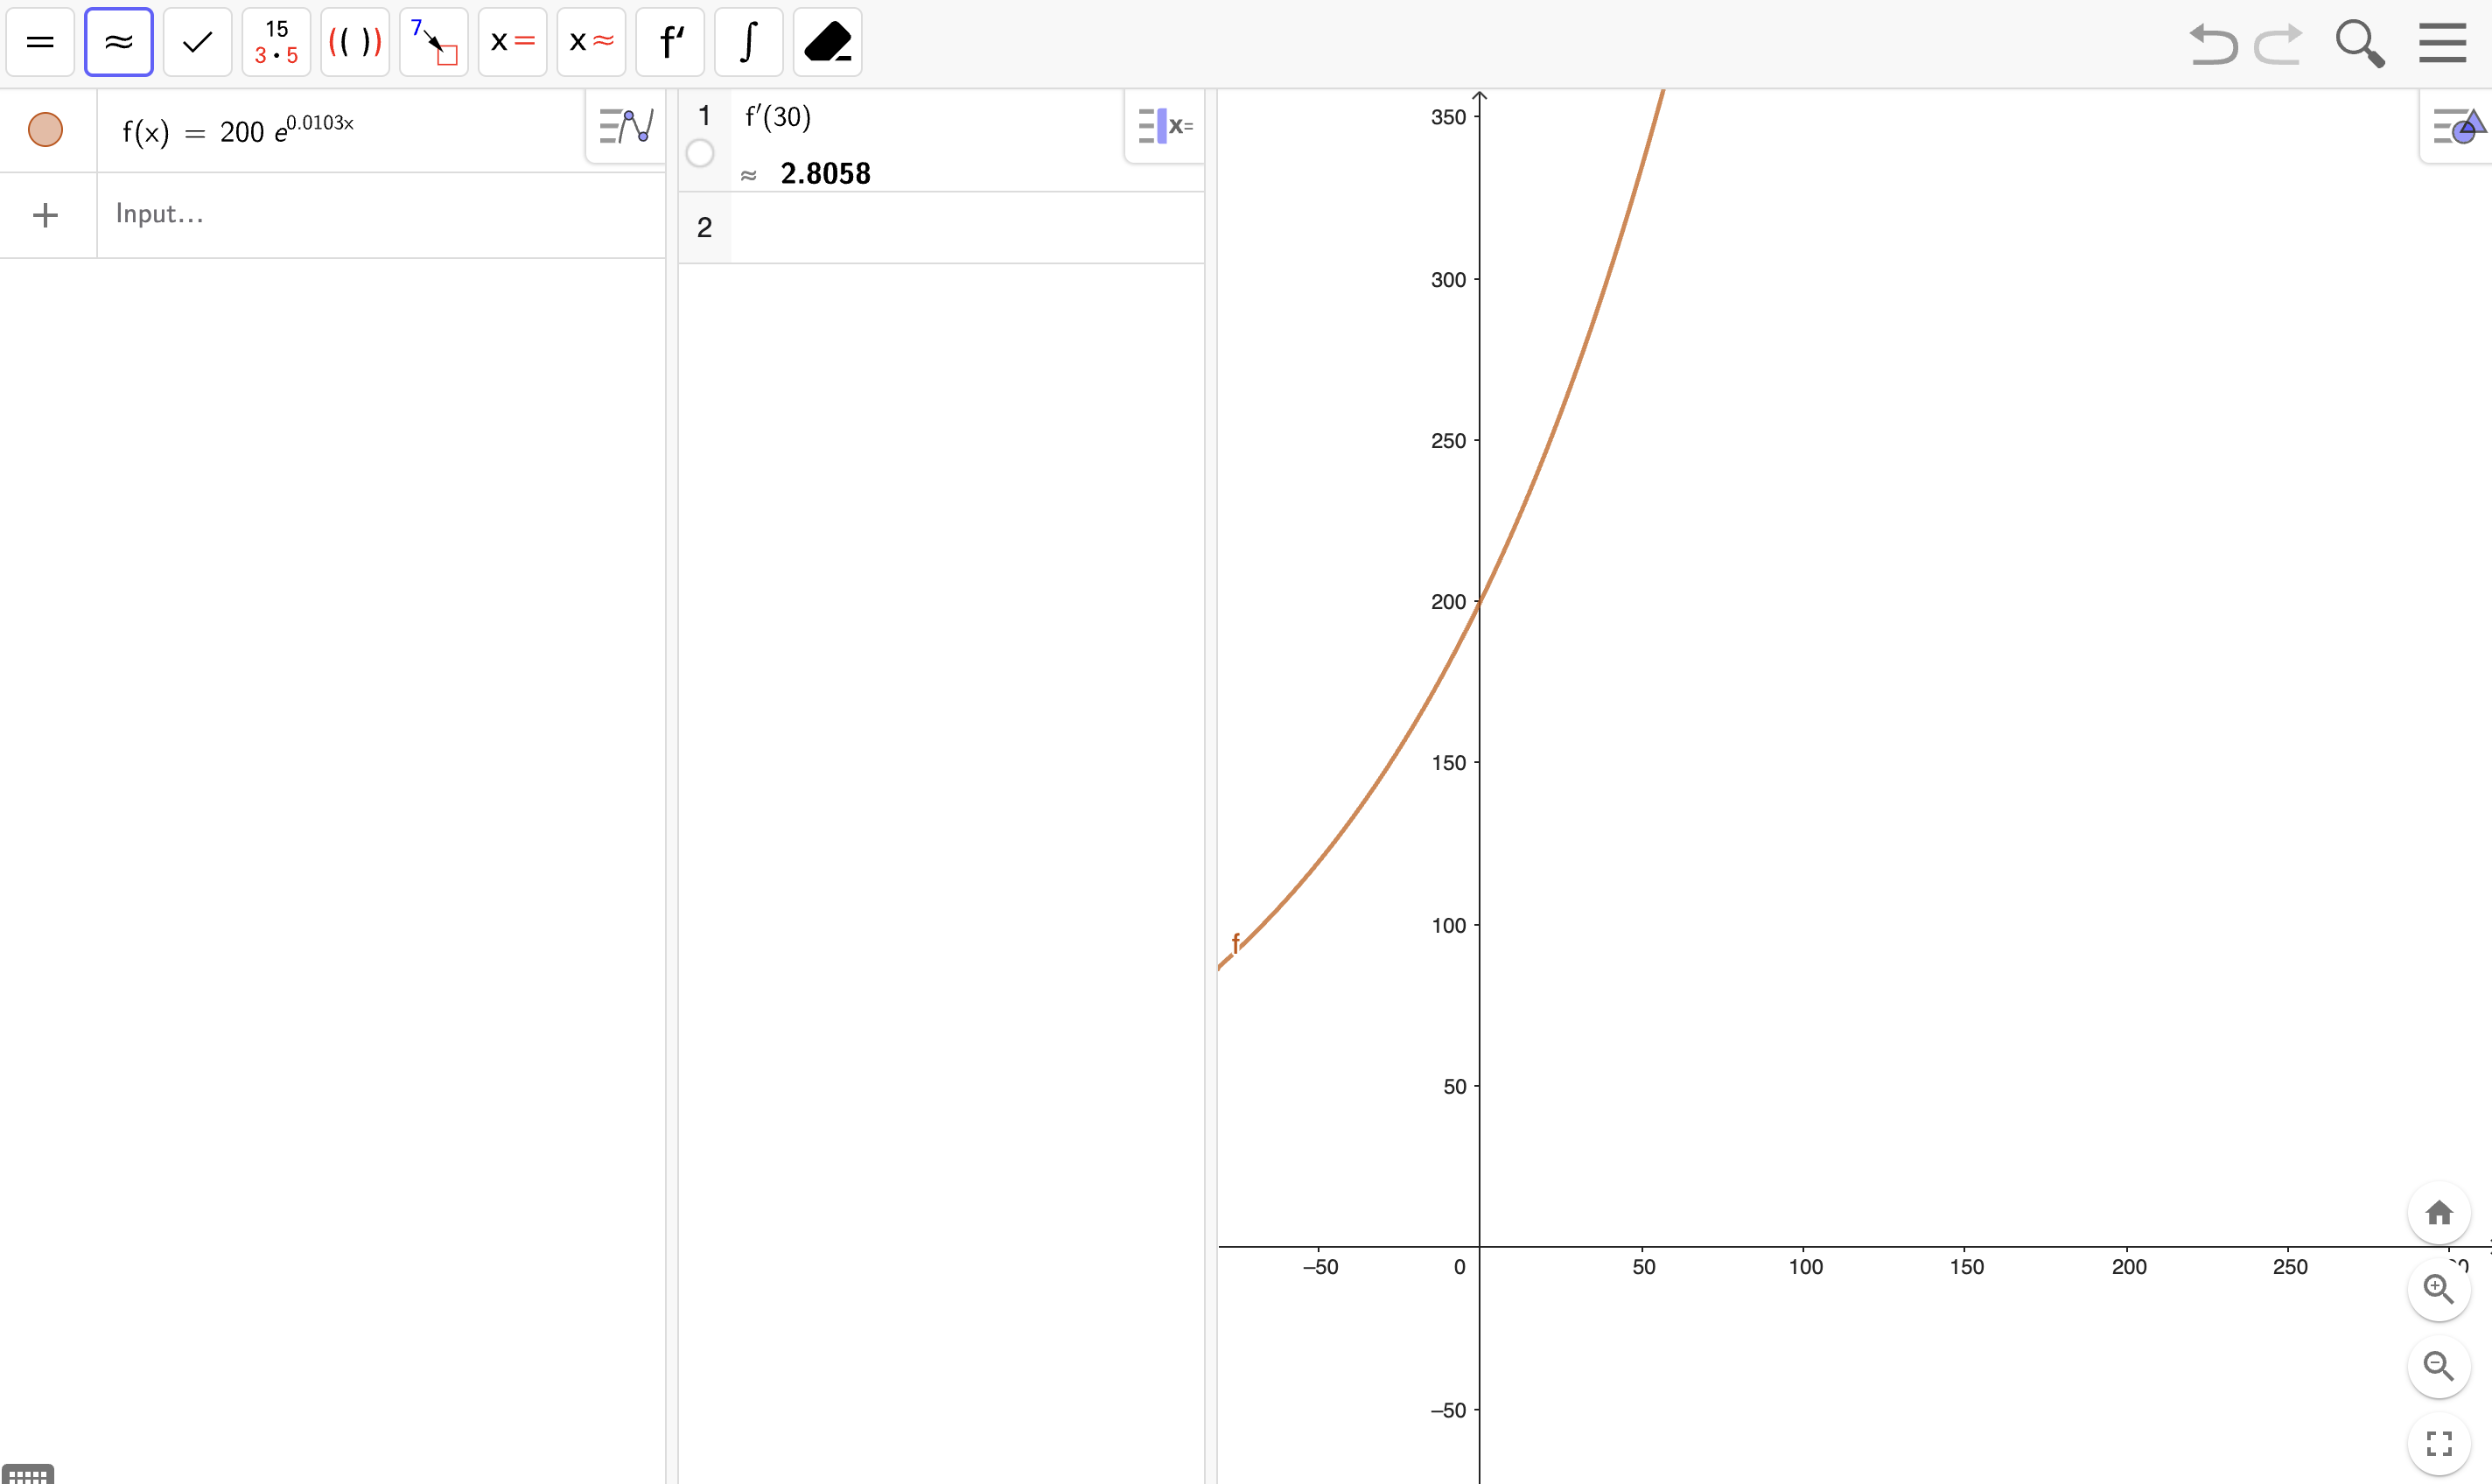
\includegraphics[width=0.8\textwidth]{afledte.png}
\end{figure}

Dvs. $f'(30)=2,8058$. Dette tal fortæller os at 30 minutter efter insprøjtningen vil styrken af strålingen stige med ca. 2.8 MBq i minuttet.

\end{enumerate}

\subsection{}
\begin{enumerate}
  \item Cirklens ligning er
    $$(x-a)^2+(y-b)^2=r^2$$
    hvor $a$ og $b$ er centrums koordinater og $r$ er radius i cirklen. Indsætter vi vores værdier får vi en ligninf for $C_1$:
    \begin{align*}
      (x-0)^2+(y-3)^2&=4^2\\
      x^2+(y-3)^2&=16
  \end{align*}

\item Med begge cirklers ligninger kan jeg indtegne dem i geogbra, finde deres skæringspunkter, og måle afstanden mellem disse punkter:
\begin{figure}[H]
\centering
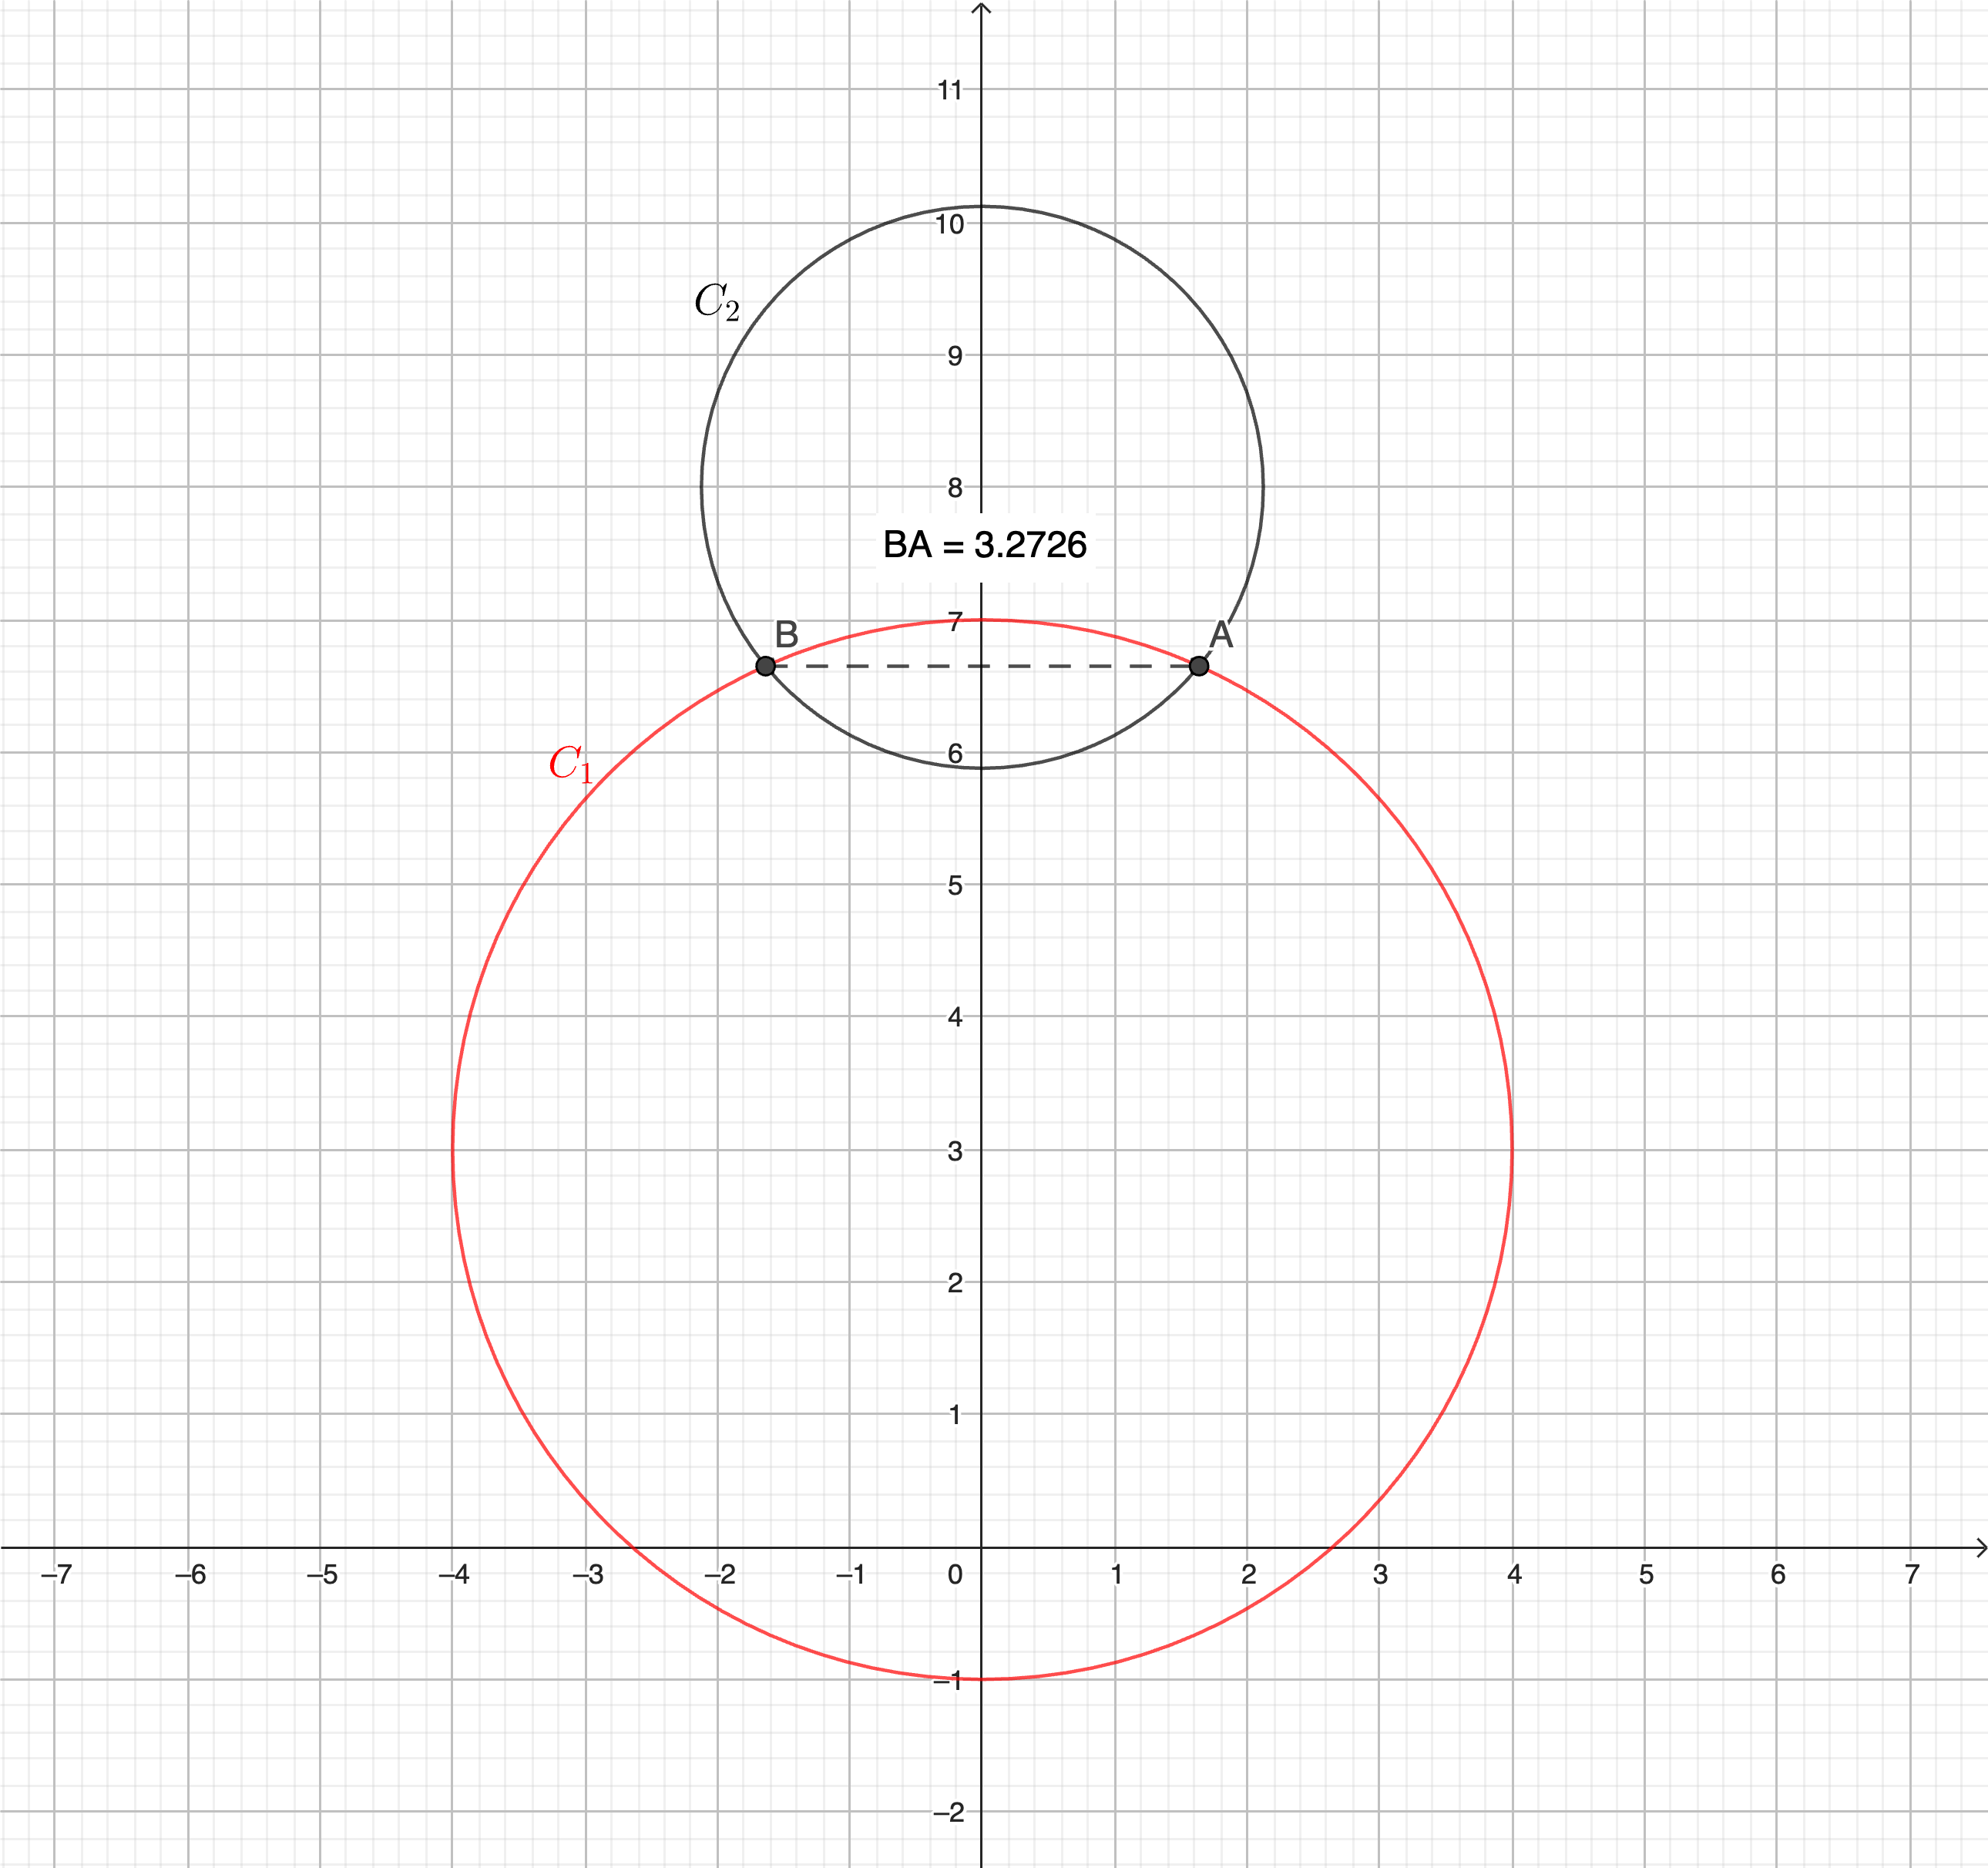
\includegraphics[width=0.7\textwidth]{flammebue.png}
\end{figure}

  \end{enumerate}

  \subsection{}
  \begin{enumerate}
    \item I denne test har vi en binomialfordeling med $n=175$ og $p=0,54$. Indtaster jeg disse værdier ind i geogebras sandsynlighedsberegner kan jeg udregne hvilke værdier for antallet af elever, som der er under 2,5\% for at få i en tilfældig udtrækning. Jeg kan her se at 82 er det første antal elever som der er over 2,5\% chance for at få i en tilfældig udtrækning:
\begin{figure}[H]
\centering
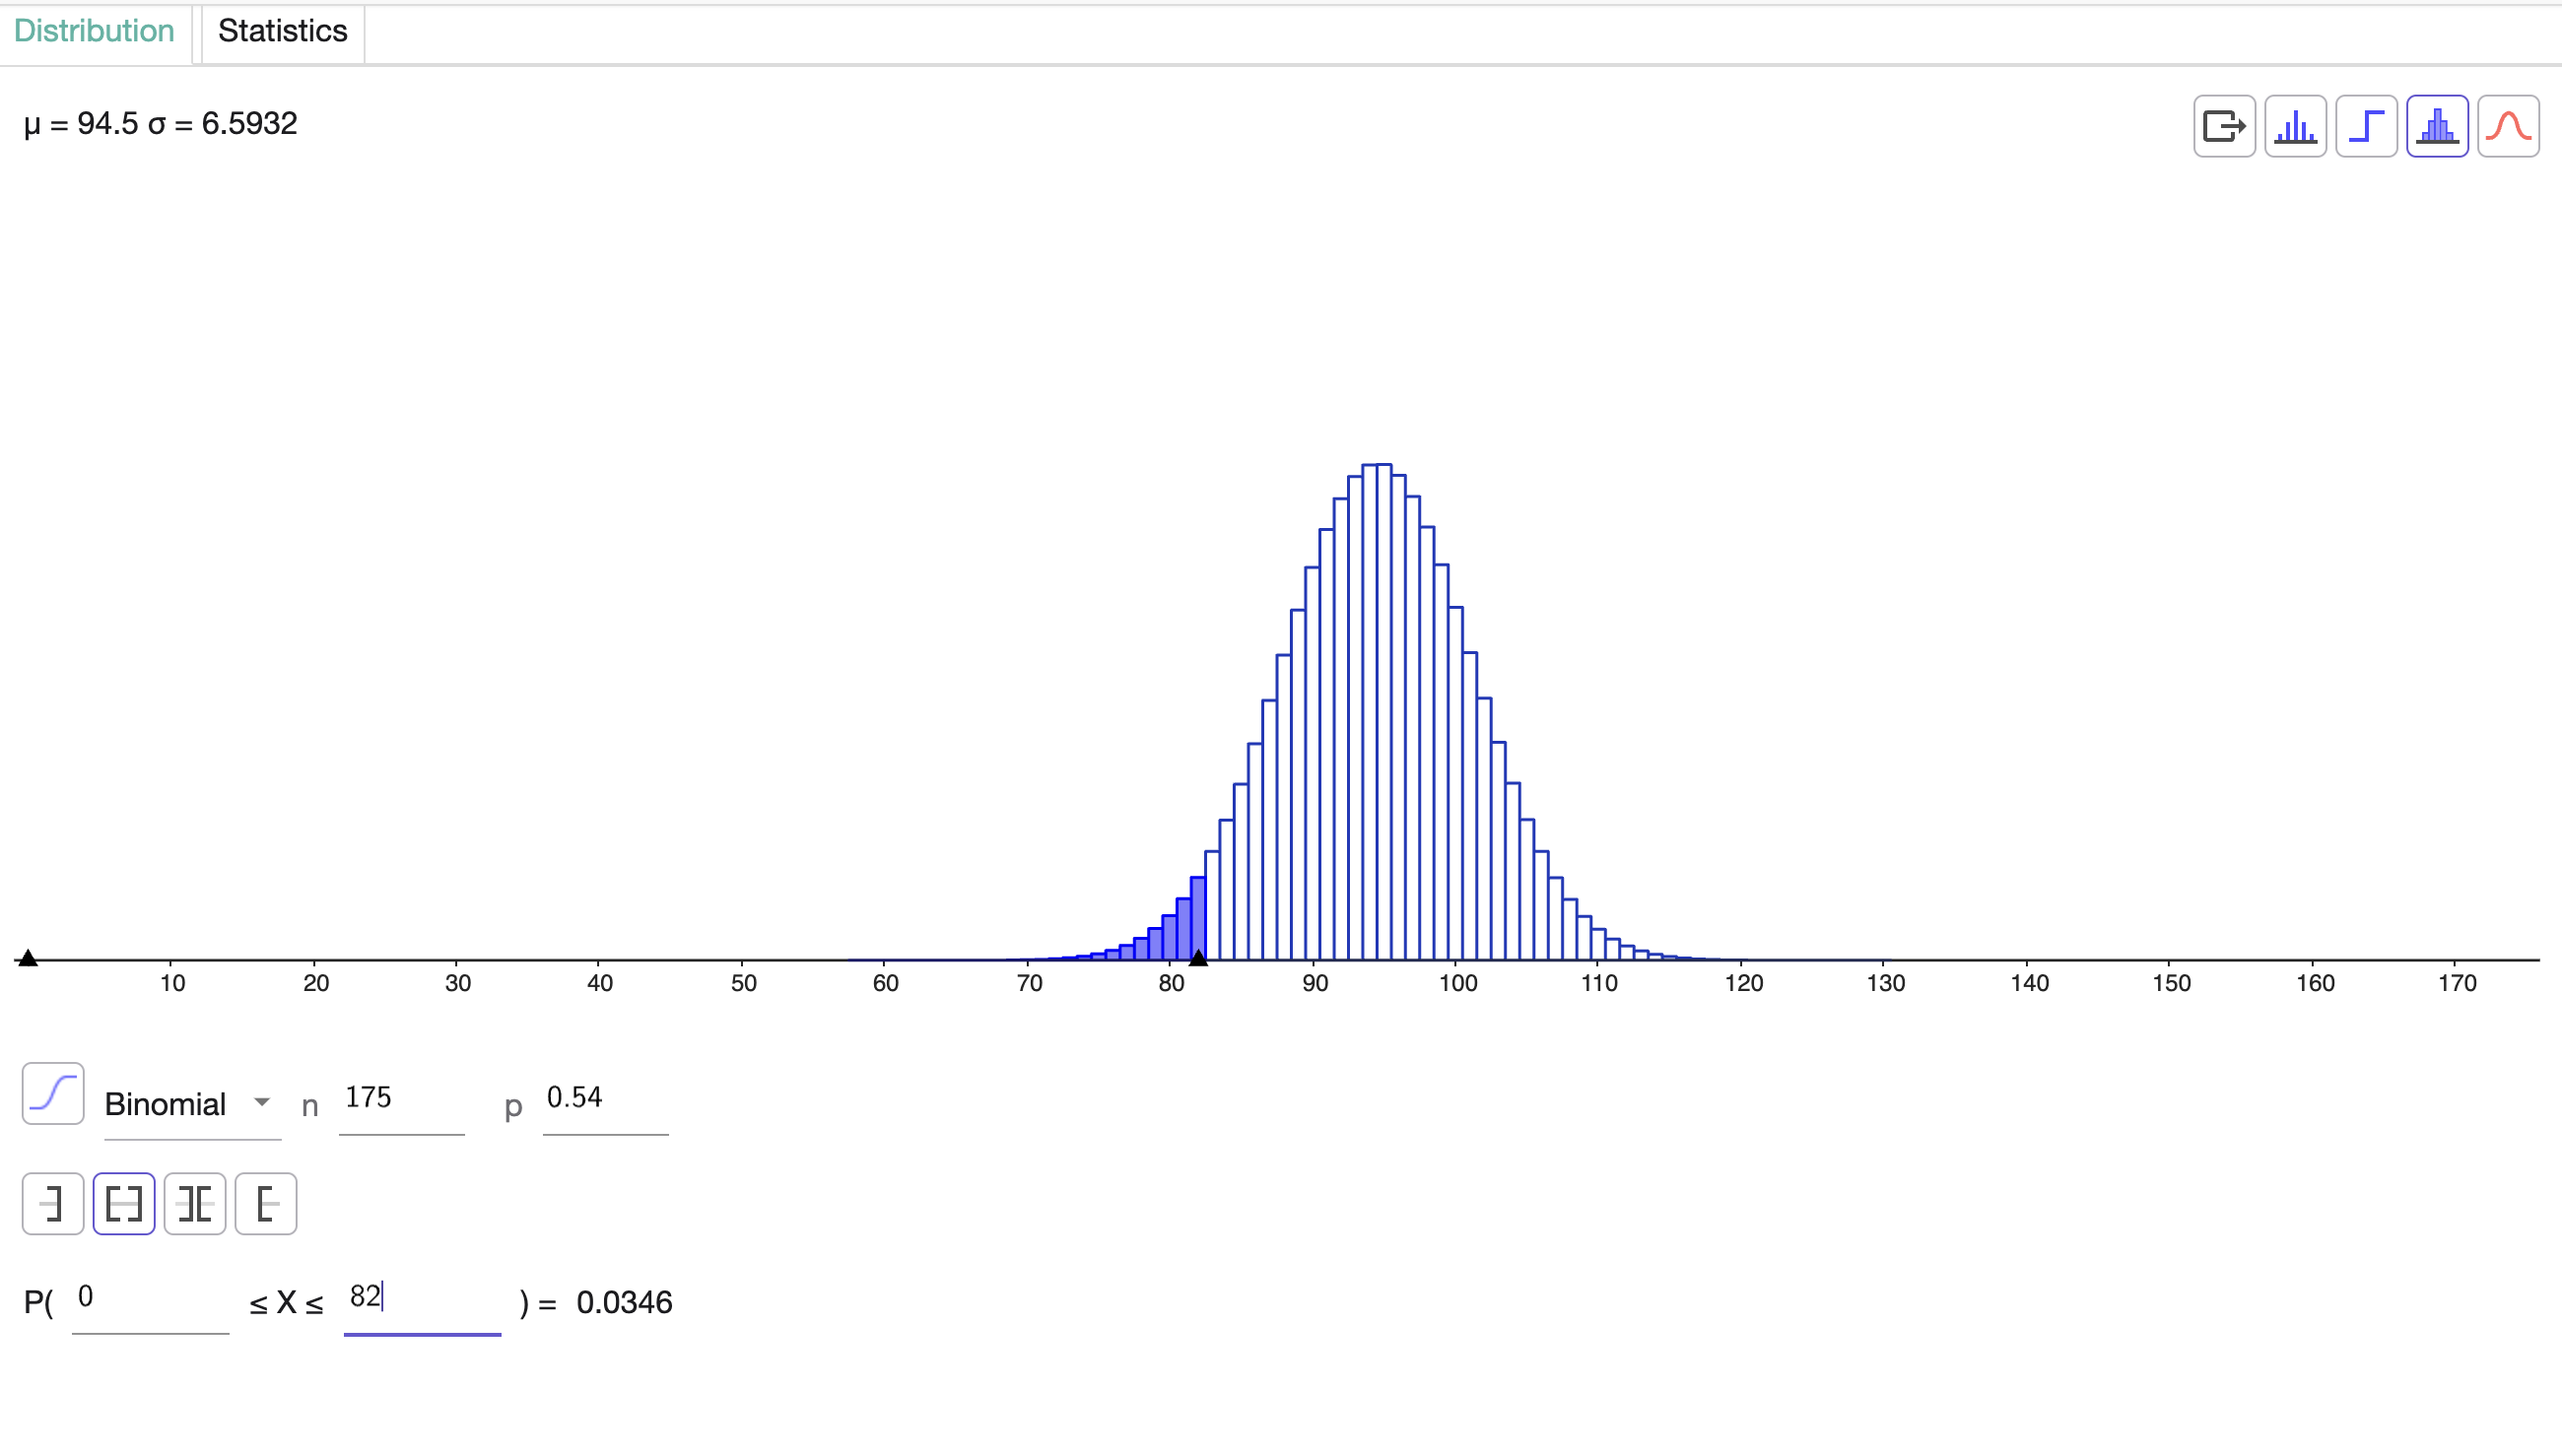
\includegraphics[width=0.7\textwidth]{biblo.png}
\end{figure}

Det sidste antal elever er 107:
\begin{figure}[H]
\centering
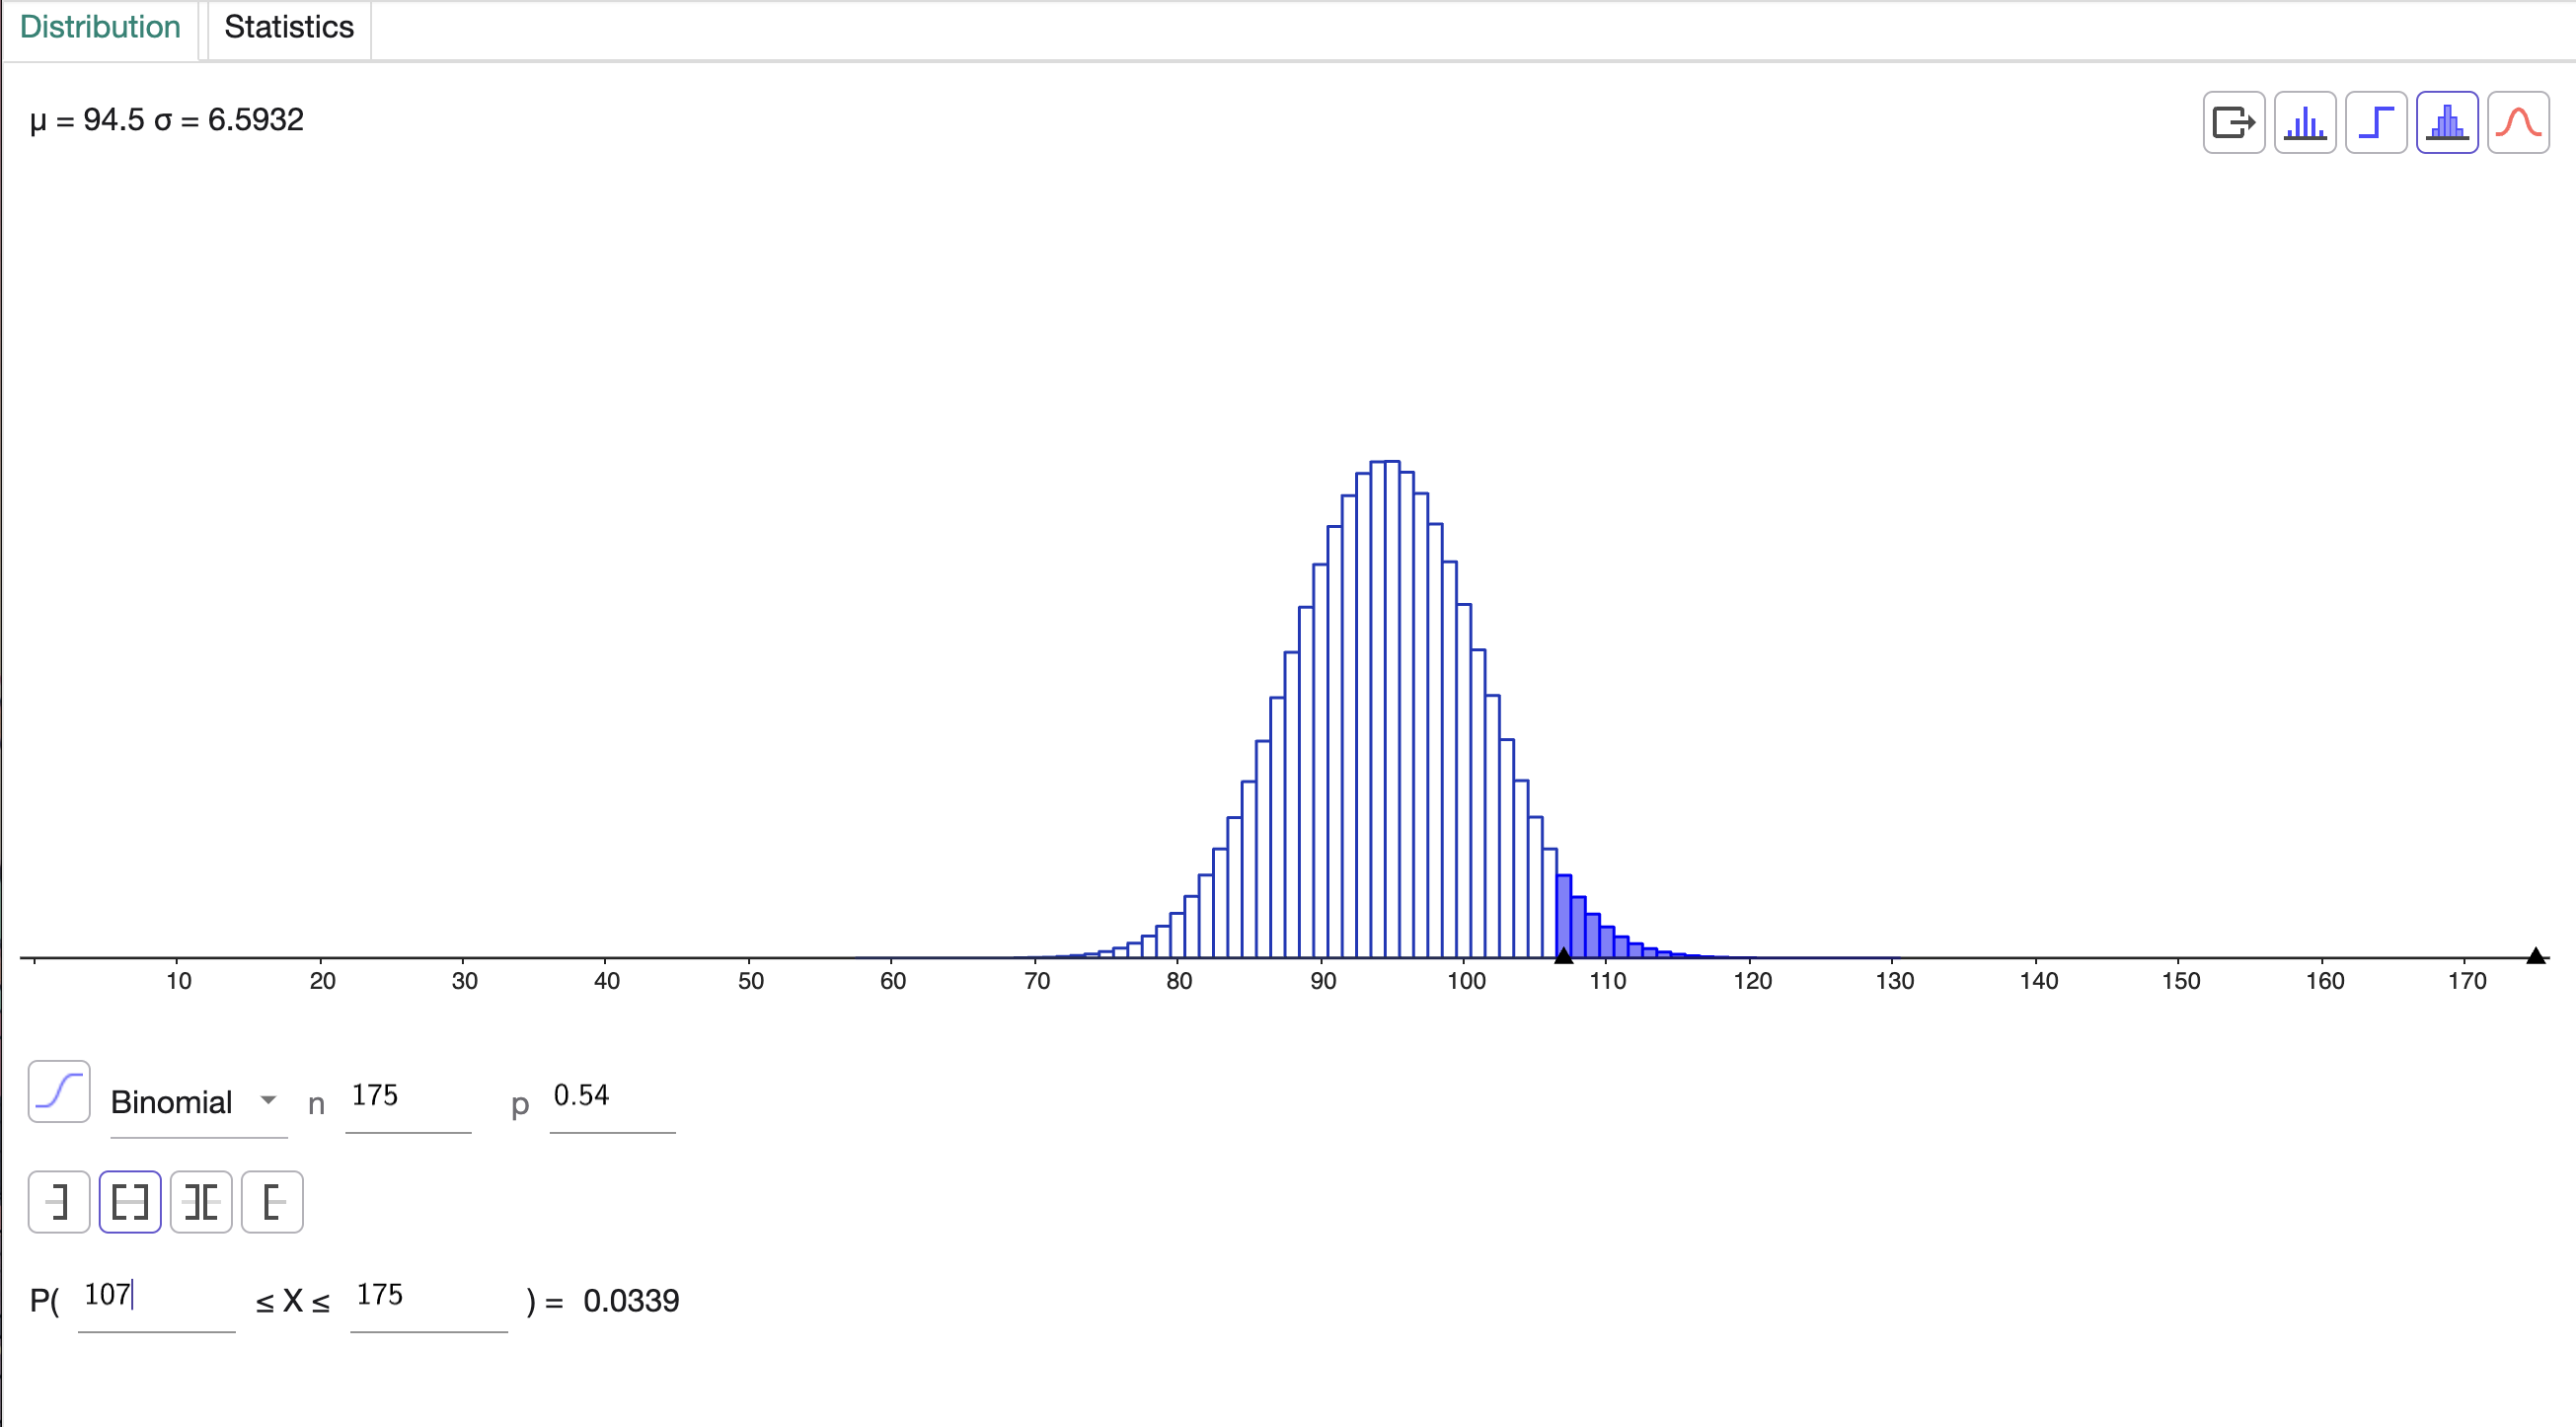
\includegraphics[width=0.7\textwidth]{biblo2.png}
\end{figure}
Acceptområdet er derfor 
$$[82;107]$$
Da den tilfældige udtrækning gav 63 elever - en værdi der altså er udenfor acceptområdet - bør nulhypotesen forkastes.

  \end{enumerate}

  \subsection{}
  \begin{enumerate}
    \item Grafen kan tegnes i geogebra:
\begin{figure}[H]
\centering
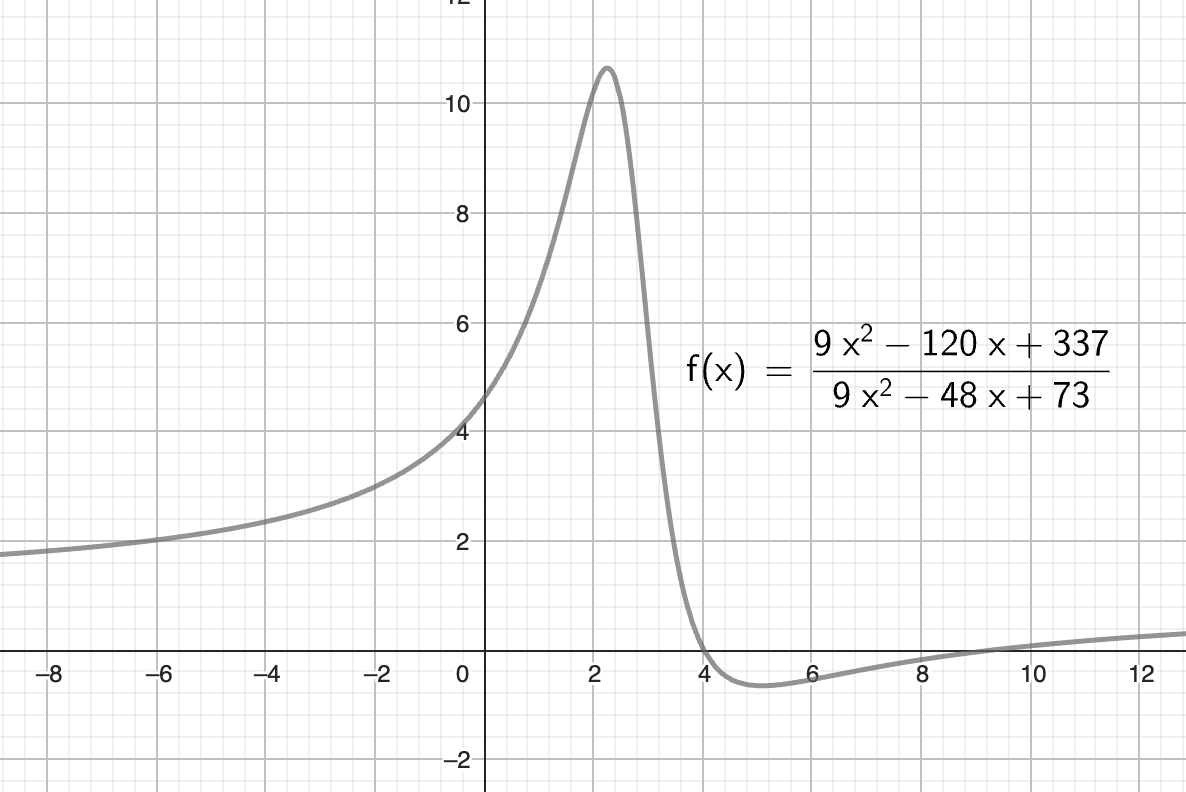
\includegraphics[width=0.8\textwidth]{grafen.png}
\end{figure}

\item Med et CAS vindue kan jeg først finde hvor denne tangent ligger på grafen ved finde $x$-værdien. Denne kan findes ved at løse $f'(x)=4$. I geogebra får jeg denne løsning til $x=1,667$.

  Dernæst kan jeg lave et punkt på grafen i geogebra og indtegne en tangent og derigennem også få dens ligning:
\begin{figure}[H]
\centering

\includegraphics[width=0.8\textwidth]{tangent.png}
\end{figure}

Denne tangents ligning er altså $y=4x+2,33$.
  \end{enumerate}

\end{document}

%%%%%%%%%%%%%%%%%%%%%%%%%%%%%%%%%%%%%%%%%%%%%%%%%%%%%%%%%%%%%%%%%%%%%%%%%%%%%% Skabeloner

% Sidestillet figur
\begin{wrapfigure}[8]{r}{0.2\textwidth}
\vspace{-18pt}
\includegraphics[width=0.3\textwidth]{ovn}
\end{wrapfigure}

% Midterstillet figur
\begin{figure}[H]
\centering
\includegraphics[width=0.8\textwidth]{abc}
\end{figure}

% Førstillet figur
\
\begin{figure}[h!]
\centering
\vspace{-15pt}
\includegraphics[width=0.35\textwidth]{stud}
\end{figure}

% Tabel
\begin{figure}[h!]
\centering\renewcommand{\arraystretch}{1.5}
\begin{tabularx}{0.9\textwidth}{|l|b|b|b|b|b|b|}
	\hline \cellcolor{hggreen} Decimaltal & 7\% & -51\% & 13,7\% & 126\% & 456\% & 0,28\%\\\hline
	\cellcolor{hggreen} Procenttal &  &  &  &  &  & \\\hline
\end{tabularx}
\end{figure}

% Forklaringsopgaver
\begin{align*}
&&	&						&&\underset{\rule{0.8\linewidth}{0pt}}{\textbf{Forklaring:}}\\[1em]
&&	&\frac{(x+2)^2 - 4}{x} 		&&\underset{\rule{0.8\linewidth}{0.4pt}}{\text{Udtrykket skrives op.}}\\[2em]
&&	=&\ \frac{x^2 + 4 + 4x - 4}{x}	&&\underset{\rule{0.8\linewidth}{0.4pt}}{\text{}}\\[2em]
&&	=&\ \frac{x^2 + 4x}{x}			&&\underset{\rule{0.8\linewidth}{0.4pt}}{\text{}}\\[2em]
&&	=&\ x + 4					&&\underset{\rule{0.8\linewidth}{0.4pt}}{\text{}}\\[2em]
\end{align*}

% Sørg for at figur er placeret før et vidst sted
\FloatBarrier




